% IEEE PacificVis 2027 -- Conference Paper Track. VGTC conference template (2024.02.14).
% Compile with pdfLaTeX + BibTeX (e.g., upload the folder to Overleaf).
% Numbers come from prototypes/paper_numbers.py; full proofs in the supplement (paper/proofs.tex).
% TODO before submission: rerun on the CDS ERA5 file; /aris:citation-audit; remove \todo notes; check 9-page limit.

\documentclass[review]{vgtc}                 % review version (double blind)
%\documentclass{vgtc}                         % final (conference style)

\ifpdf%
  \pdfoutput=1\relax
  \pdfcompresslevel=9
  \pdfoptionpdfminorversion=7
  \ExecuteOptions{pdftex}
  \usepackage{graphicx}
  \DeclareGraphicsExtensions{.pdf,.png,.jpg,.jpeg}
\else%
  \ExecuteOptions{dvips}
  \usepackage{graphicx}
  \DeclareGraphicsExtensions{.eps}
\fi%

\graphicspath{{figures/}}
\usepackage{times}
\renewcommand*\ttdefault{txtt}
\usepackage{booktabs}
\usepackage{mathptmx}
\usepackage{amsmath,amssymb,amsthm}
\usepackage{xcolor}
\usepackage{algorithm}
\usepackage[noend]{algpseudocode}
\newcommand{\todo}[1]{\textcolor{red}{[TODO: #1]}}
\newtheorem{theorem}{Theorem}
\newtheorem{proposition}{Proposition}
\newtheorem{corollary}{Corollary}
\newtheorem{definition}{Definition}

\onlineid{0}          % TODO: replace with the submission ID
\vgtccategory{Research}
\vgtcinsertpkg

\title{How Faithful Can a Hierarchy-Constrained 1-D Layout Be?\\Certified Position--Topology Trade-offs for Merge Tree Maps and Beyond}

\author{Anonymous Authors}   % double-blind review

\teaser{
  \centering
  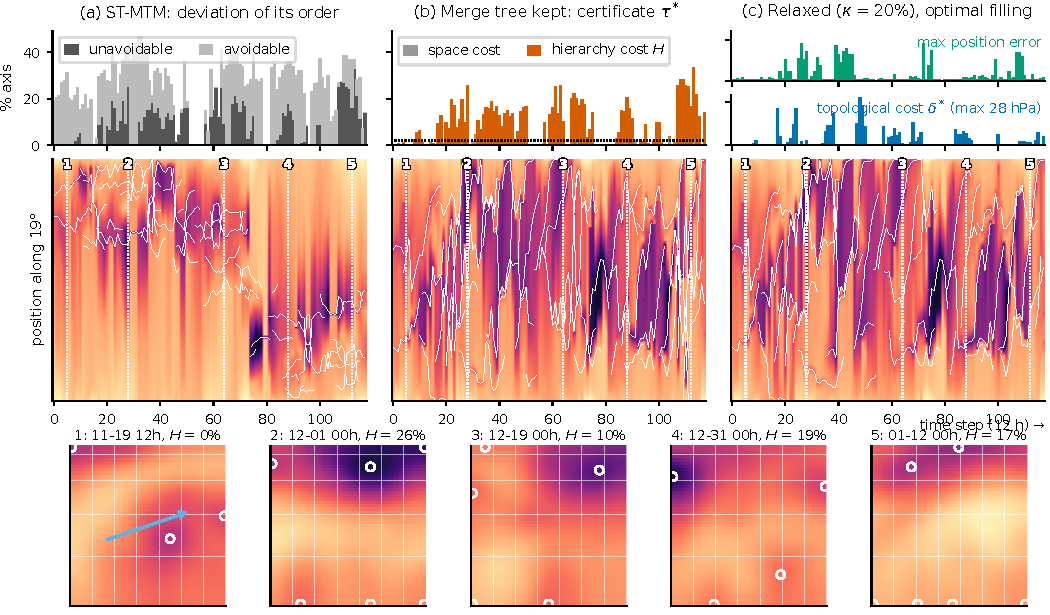
\includegraphics[width=\linewidth]{fig_teaser}
  \caption{Merge tree maps of 59 days of ERA5 sea-level pressure over Europe (columns: 12-hourly time steps; white lines: tracked pressure lows; vertical axis: principal direction of their motion). (a) ST-MTM keeps the merge tree. Strip: per time step, the deviation of its leaf order from the lows' positions under the best monotone reading of its axis (light), and the part that \emph{no} merge-tree-preserving order can avoid (dark; width-free certificate, \cref{sec:cert}). (b) Anchored layout that keeps the merge tree and attains the certificate $\tau^*$; orange: hierarchy cost. (c) Certificate-driven relaxation rendered with the optimal filling: the mean maximum position error drops from 9.6\% to 3.5\% of the axis, at an exact, displayed per-frame topological cost $\delta^*$ (blue, hPa).}
  \label{fig:teaser}
}

\abstract{
Static space--time visualizations compress each time step of a 2-D field into a 1-D column and stack the columns over time. Their 1-D order is often constrained by a hierarchy: merge tree maps keep every merge-tree subtree contiguous, and dendrogram-ordered pixel displays keep every cluster contiguous. When the hierarchy disagrees with space, every admissible layout must misplace some feature, yet existing quality measures describe the layout at hand rather than the error that no layout can avoid. We model such maps as hierarchy-constrained 1-D interval layouts and show that (i) the minimum achievable maximum deviation from a positional reference has a closed form for a fixed order, decomposes into a hierarchy and a space component, and is computable at display resolution by an exact pseudo-polynomial dynamic program; (ii) for any 1-D map and any scalar filling, breaking the contiguity of a subtree distorts merge levels by at least half the gap between the subtree's merge value and its parent's, a distortion that equals the labelled interleaving distance under standard conventions; and the smallest such distortion over all fillings of a given order has a closed form attained by a barrier filling; (iii) since positions and merge levels depend on the order only through these two closed forms, the exact position--topology frontier of all 1-D maps is computable for small trees, with a certified lower bound for large ones. A width-free variant of the certificate applies to every merge tree map, whatever its width model. On three real datasets from two domains, hierarchy-induced conflicts occur in 58--63\% of time steps under an automatic reference direction, also without widths, and in 23--77\% across fixed directions. In a geometric reader proxy, the vertical distance changes of existing merge tree maps have the opposite sign of the true approach or separation of feature pairs in 21--34\% of clear cases; a certificate-driven relaxation lowers this to 4--15\% at an exact topological cost and lies on the exact frontier in 98\% of time steps. The certificate also transfers to 1024-leaf dendrogram displays.
}

\keywords{Merge trees, hierarchy-constrained layout, time-varying scalar fields, static visualization, faithfulness, interleaving distance.}

\begin{document}

\firstsection{Introduction}
\maketitle

A static summary shows the complete evolution of spatio-temporal data in a single image, complementing animation, which is transient and hard to compare over time. Hovm\"oller diagrams track weather systems along a fixed longitude or latitude~\cite{Hovmoller:1949}; dense pixel displays and MotionRugs arrange entities as pixel columns over time~\cite{Keim:2000:PIX,Buchmueller:2019:MR}; 1-D projections support the analysis of spatio-temporal phenomena~\cite{Franke:2021:1DP}; merge tree maps linearize each time step of a scalar field while preserving its merge tree~\cite{Koepp:2023:TMTM,STMTM:2026}. All of them compress space to one axis and put time on the other, and readers infer spatial proximity and motion from vertical proximity.

These displays share a second property: \emph{their 1-D order is constrained by a hierarchy}. Merge tree maps keep the leaves of every merge-tree subtree contiguous, which keeps features intact and preserves the merge tree~\cite{Koepp:2023:TMTM}. Clustered heatmaps~\cite{Eisen:1998:CA} and hierarchical orderings of pixel displays~\cite{Franke:2021:1DP} keep clusters contiguous. Geophylogenies align tree-constrained leaf orders with map sites~\cite{Klawitter:2025:GP}. Hierarchy and space need not agree. Two pressure lows may merge first because they share a trough, while an unrelated third low lies geographically between them (\cref{fig:toy}). Then every admissible layout misplaces some feature.

Abstract views are known to mislead~\cite{McNutt:2020:SVM,Wattenberg:2016:TSNE}, and projection quality is routinely measured~\cite{Venna:2001:NP,Aupetit:2007:VD}. ST-MTM reports distance stress and neighbourhood preservation and discusses that no 1-D order preserves all distances~\cite{STMTM:2026}. Such measures describe the layout that was produced. No method certifies the \emph{unavoidable} maximum deviation from a positional reference, nor states how much hierarchy information must be given up to reduce it. The consequence is concrete: in a geometric reader proxy on ERA5 sea-level pressure (RQ2 in \cref{sec:eval}), the vertical distance change of two lows on a temporal merge tree map has the opposite sign of their true 24-hour approach or separation in 33.7\% of clear cases (permutation null 39.7\%), and 24.9\% on ST-MTM.

We ask: \textbf{how faithful to a positional reference can a hierarchy-constrained 1-D layout be, and can its unfaithfulness be certified, located, and controlled?} Following the argument that visualization quality must be defined before it can be measured and guaranteed~\cite{Meulemans:2026:AP}, we do not propose yet another layout, but a certified bound and a controlled trade-off. Our contributions are:
\begin{itemize}
\item \textbf{A positional certificate} for hierarchy-constrained 1-D interval layouts: a closed form for fixed orders, a decomposition into hierarchy and space costs, explanatory witness triples, and an exact pseudo-polynomial dynamic program at display resolution (\cref{sec:model,sec:cert}).
\item \textbf{A width-free certificate} that bounds every merge tree map under any monotone reading of its axis (\cref{sec:cert}).
\item \textbf{A filling-independent topological price} of breaking contiguity, its interpretation as the labelled interleaving distance, the \textbf{optimal filling} of any order in closed form, and the resulting \textbf{exact position--topology frontier} with a scalable certified lower bound; a threshold-and-prune relaxation that lies on the exact frontier in 98\% of time steps (\cref{sec:topo}).
\item \textbf{A cross-domain characterization} on three real and two synthetic datasets, and a concrete design use on dendrogram-ordered pixel displays (\cref{sec:eval}).
\end{itemize}

\section{Related Work}

\textbf{Static summaries of spatio-temporal data.}
Hovm\"oller and radius--time diagrams aggregate or slice the orthogonal dimension and thereby merge distinct features. Space-filling curves~\cite{Franke:2021:1DP,Zhou:2021:DSF} and pixel-oriented techniques~\cite{Keim:2000:PIX} linearize densely; Keim framed pixel arrangement as an optimization problem. MotionRugs~\cite{Buchmueller:2019:MR}, stable visual summaries~\cite{Wulms:2021:SVS}, MoReVis~\cite{Valdrighi:2024:MRV}, and GroupRugs~\cite{Stolk:2025:GR} target trajectories and regions. GroupRugs keeps groups contiguous and evaluates spatial quality, stability, and expressiveness with neighbourhood-based ordering measures; it provides no bound on the conflict between grouping and space. Topological landscapes~\cite{Weber:2007:TL,Beketayev:2012:GPTL}, temporal merge tree maps~\cite{Koepp:2023:TMTM}, and spatiotemporal merge tree maps~\cite{STMTM:2026} preserve topology; temporal treemaps and nested tracking graphs lay out evolving hierarchies~\cite{Koepp:2019:TT,Lukasczyk:2017:NTG}.

\textbf{Hierarchy-constrained orders.}
Optimal leaf ordering~\cite{BarJoseph:2001:OLO} underlies clustered heatmaps~\cite{Eisen:1998:CA}. Tree-constrained leaf orders against external positions appear in geophylogenies~\cite{Klawitter:2025:GP}, external-order rearrangement~\cite{Bulteau:2022:RT}, and displacement-optimized tanglegrams~\cite{Huson:2026:DOT}, with crossing, inversion, or summed-displacement objectives.

\textbf{Faithfulness, distortion, and trade-offs.}
Visualization mirages~\cite{McNutt:2020:SVM} and misread embeddings~\cite{Wattenberg:2016:TSNE} show how abstract views mislead; trustworthiness and continuity~\cite{Venna:2001:NP} and distortion maps~\cite{Aupetit:2007:VD,Rauscher:2025:1DO,Rauscher:2026:VB} measure and display projection artefacts. Cartograms trade area, shape, and topology errors~\cite{Nusrat:2016:CART}; data--spatial grid maps interpolate between spatial and data layouts~\cite{vanBeusekom:2023:DSL}; spatially ordered treemaps measure positional consistency of hierarchical layouts~\cite{Wood:2008:SOT}. Kindlmann and Scheidegger formalize visual--data correspondence~\cite{Kindlmann:2014:AVD}.

\textbf{1-D placement.}
Without a hierarchy, minimizing the maximum displacement needed to separate intervals on a line is solvable in $O(n\log n)$~\cite{Li:2019:SOI}; this is the free case of our certificate (without our canvas and eccentricity constraints). Separation-constrained quadratic programs are standard in constrained graph layout~\cite{Dwyer:2006:IPSEP}.

\textbf{Merge tree distances.}
Interleaving distances compare merge trees~\cite{Morozov:2013:IDMT}; the $\ell_\infty$-cophenetic metric of labelled trees is an interleaving distance~\cite{Munch:2019:LINF}; intrinsic and geometry-aware interleavings and Wasserstein metrics support comparison, tracking, and averaging of time-varying data~\cite{Gasparovic:2024:IID,Yan:2022:GAMT,Pont:2022:WMT}, including cyclones and atmospheric rivers~\cite{Yan:2024:TROPHY,Lan:2024:AR}. To our knowledge, interleaving distances have not been used to evaluate layouts; we use them to measure what a 1-D map does to the merge tree.

\section{Problem and Motivation}\label{sec:model}

\begin{figure*}[t]
\centering
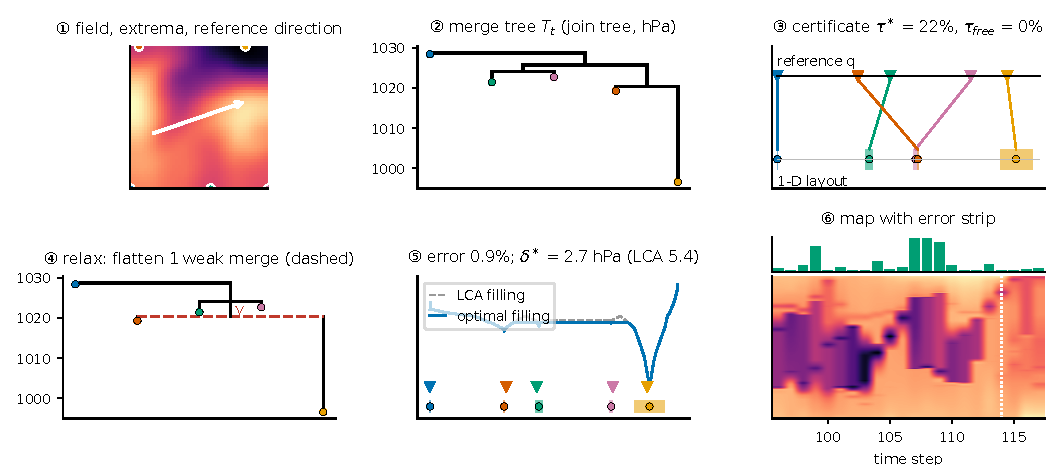
\includegraphics[width=\linewidth]{fig_pipeline}
\caption{Method overview on one ERA5 time step (2000-01-13 00\,UTC, five pressure lows). \textcircled{\scriptsize 1} Extrema and the automatic reference direction. \textcircled{\scriptsize 2} Merge tree. \textcircled{\scriptsize 3} Certificate: the best merge-tree-preserving layout must deviate by $\tau^*=22\%$ of the axis, whereas an unconstrained order needs 0\%; the hierarchy cost exceeds $\theta$. \textcircled{\scriptsize 4} The threshold-and-prune relaxation flattens one weak merge (dashed), so its leaves may interleave with others. \textcircled{\scriptsize 5} The relaxed layout deviates by 0.9\%; the optimal barrier filling limits the merge-level distortion to $\delta^*=2.7$\,hPa, half that of the LCA filling. \textcircled{\scriptsize 6} The map shows each column's error and $\delta^*$ in strips.}
\label{fig:pipeline}
\end{figure*}

\textbf{Merge tree maps.}
For each time step $t$, the leaves of the merge tree $T_t$ (a join tree for pressure minima, a split tree for fire intensity maxima) are features with extremum position $R_i$, support measure $A_i$, and pairwise merge values $f(\mathrm{lca}(i,j))$. A map chooses a leaf order, an interval per leaf, and an anchor (the extremum position) inside the interval; fills the column along leaf arcs and lowest-common-ancestor paths~\cite{Koepp:2023:TMTM,STMTM:2026}; and stacks columns over time.

\textbf{A natural remedy.}
Readers ask where features are and where they move. The natural remedy is to anchor each feature to a reference coordinate $q_i=\varphi(R_i)$ and solve, over all hierarchy-consistent orders, a linear program for the smallest maximum deviation, followed by a budgeted quadratic program balancing reference error, distance stress, motion residual, and eccentricity. We call this the \emph{reference-anchored layout}; it is part of our method.

\textbf{It is not enough.}
Even the optimal reference-anchored layout deviates by more than 2\% of the axis in 58\% of ERA5 frames (up to 31\%), and in the reader proxy it performs like ST-MTM (22.4\% vs.\ 24.9\% reversals). The obstacle is the hierarchy itself, which raises our questions: how large must the deviation be, what causes it, and what does relaxing the hierarchy cost?

\textbf{Model.}
Let the hierarchy be a rooted tree $T$ with leaves $1,\dots,n$. Leaf $i$ has reference $q_i$, width $w_i=cA_i$ with $c$ fixed over time, and eccentricity radius $h_i=\rho w_i/2$, $\rho\in[0,1]$; let $g$ be a minimum gap and $[a,a+L]$ the canvas. A layout $(\pi,z,u)$ consists of a leaf order, interval centres, and anchors satisfying
(H) $\pi\in\Pi(T)$, i.e., every node's leaf set $S_v$ is contiguous in $\pi$;
(D) $z_y-z_x\ge (w_x+w_y)/2+g$ for $\pi$-consecutive $x,y$;
(C) $a+w_i/2\le z_i\le a+L-w_i/2$;
(E) $|u_i-z_i|\le h_i$.
Legal orders arise by permuting children blocks at every node, so $|\Pi(T)|=\prod_v\deg(v)!$. We distinguish three fidelities: \emph{position} ($u_i-q_i$), \emph{size} (widths proportional to measure and comparable over time), and \emph{topology} (merge levels of the rendered map, \cref{sec:topo}). TMTM preserves topology and absolute size but does not control position; ST-MTM preserves topology and relative distances and fits target width shares; the reference-anchored layout targets position under the hierarchy.

\begin{figure}[t]
\centering
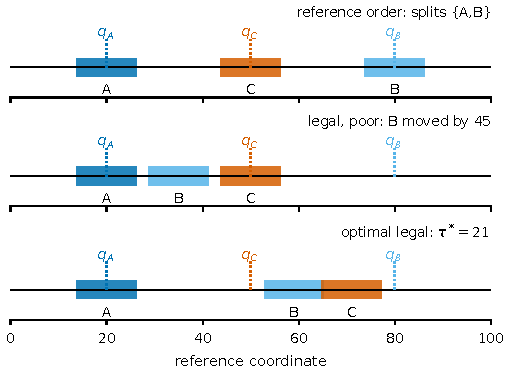
\includegraphics[width=\linewidth]{fig_toy_conflict}
\caption{Three-leaf conflict with tree $((A,B),C)$. Sorting by reference splits subtree $\{A,B\}$ (left); a legal but poor layout (middle); the optimal legal layout has maximum deviation $\tau^*=21=(q_B-q_C+w)/2$, split between $B$ and $C$ (right).}
\label{fig:toy}
\end{figure}

\section{A Positional Certificate}\label{sec:cert}

\begin{definition}
$\tau(\pi)=\min_{z,u}\max_i|u_i-q_i|$ subject to (D)(C)(E); $\tau^*(T)=\min_{\pi\in\Pi(T)}\tau(\pi)$; $\tau_{\rm free}$ is the same minimum over all permutations; the \emph{hierarchy cost} is $H=\tau^*-\tau_{\rm free}$ and the \emph{space cost} is $\tau_{\rm free}$.
\end{definition}

\begin{proposition}[Closed form]\label{prop:closed}
Number the leaves along $\pi$. With $s_k=(w_k+w_{k+1})/2+g$, $S_{ij}=\sum_{k=i}^{j-1}s_k$, $D_k=\sum_{m<k}w_m+w_k/2+(k-1)g$, $E_k=\sum_{m>k}w_m+w_k/2+(n-k)g$, and capacity $\sum_iw_i+(n-1)g\le L$,
\[\tau(\pi)=\max\Big\{0,\ \max_{i<j}\tfrac{q_i-q_j+S_{ij}-h_i-h_j}{2},\ \max_k(a+D_k-q_k-h_k),\ \max_k(q_k-h_k-a-L+E_k)\Big\}.\]
\end{proposition}
Eliminating anchors turns each centre constraint into a box window $|z_k-q_k|\le\tau+h_k$; a chain with lower-bounded separations and box windows is feasible iff its earliest placement stays inside every window; expanding the resulting inequalities gives the formula. It agrees with a linear-programming solver to $2\cdot10^{-14}$.

\begin{proposition}[Monotonicity and witnesses]
Flattening a node (attaching its children to its parent) enlarges $\Pi$ and never increases $\tau^*$; flattening all nodes yields $\tau_{\rm free}$, so $H\ge0$ is exactly the price of keeping every subtree contiguous. If $i,j\in S_v$, $k\notin S_v$ and $q_i<q_k<q_j$, then $\tau^*\ge\frac12\min(q_k-q_i,\,q_j-q_k)$.
\end{proposition}
The witness triple explains \emph{which} features conflict and can be highlighted in the display. In \cref{fig:toy}, the witness bound is 15 and $\tau^*=21$.

\textbf{Exact computation at display resolution.}
Enumerating $\Pi(T)$ is exponential. Discretize the canvas into $N$ pixels with integer widths $W_i$ and gap $G$, and let $E_S(x)$ be the earliest start available after placing all leaves of subtree $S$ in a legal order with no start before $x$.

\begin{theorem}[Exact dynamic program]\label{thm:dp}
For a leaf, $E_i(x)=\max(x,lo_i)+W_i+G$, or $\infty$ if $\max(x,lo_i)>hi_i$ (the window of Proposition~\ref{prop:closed}); for a binary node, $E_S=\min(E_B\circ E_A,\ E_A\circ E_B)$; for an $m$-ary node, a subset recursion over children. A deviation $\tau$ is feasible iff $E_{\rm root}(0)<\infty$. Bisection yields $\tau^*$ to a given tolerance in $O(nN\log(N/\varepsilon))$ time for binary hierarchies---pseudo-polynomial in $N$---and $O(2^m mN)$ per $m$-ary node.
\end{theorem}
Correctness rests on an earliest-completion argument: for a fixed order, greedy earliest placement minimizes every start, so a block passes only its earliest next start to the rest of the chain, and smaller is never worse. \Cref{alg:cert} lists the computation.

\begin{algorithm}[t]
\caption{Certificate $\tau^*$ at display resolution (Theorem~\ref{thm:dp}).}\label{alg:cert}
\begin{algorithmic}[1]
\Require hierarchy $T$; pixel widths $W_i$, gap $G$, references $q_i$, radii $h_i$; $N$ pixels; tolerance $\varepsilon$
\Function{Earliest}{$S,\tau$} \Comment{array over starts $x=0,\dots,N$}
  \If{$S$ is a leaf $i$}
    \State $lo_i\gets\lceil q_i-\tau-h_i-W_i/2\rceil$, $hi_i\gets\lfloor q_i+\tau+h_i-W_i/2\rfloor$
    \State \Return $x\mapsto\max(x,lo_i)+W_i+G$ if $\max(x,lo_i)\le hi_i$, else $\infty$
  \EndIf
  \State $E_c\gets$ \Call{Earliest}{$c,\tau$} for every child $c$ of $S$
  \State $F_\emptyset\gets\mathrm{id}$;\ \ $F_M\gets\min_{c\in M}E_c\circ F_{M\setminus\{c\}}$ for all subsets $M$ of children
  \State \Return $F_{\rm all\ children}$ \Comment{binary: $\min(E_B\circ E_A,\,E_A\circ E_B)$}
\EndFunction
\State $\tau^*\gets$ smallest $\tau$ with \Call{Earliest}{root$,\tau$}$(0)<\infty$, by bisection to $\varepsilon$
\end{algorithmic}
\end{algorithm}

\begin{proposition}[Certified lower bound]\label{prop:lb}
If widths and gap are integer pixels, $0\le\tau^*_{\rm disc}-\tau^*_{\rm cont}\le\delta/2$ for pixel size $\delta$. For real widths, rounding widths and gap \emph{down} while keeping the slacks gives $\tau^*_{\rm cont}\ge\tau^*_{\rm disc,relax}-\delta/2$.
\end{proposition}
\textbf{A width-free certificate.}
Other merge tree maps use other width models: TMTM allocates one pixel per sample, and ST-MTM fits target widths. Dropping widths, gaps, eccentricity, and canvas removes all constraints but the order.

\begin{proposition}[Width-free certificate]\label{prop:pt}
Let $\tau_{\rm pt}(\pi)=\max\{0,\max_{i\text{ before }j}(q_i-q_j)/2\}$ and $\tau^*_{\rm pt}=\min_{\pi\in\Pi(T)}\tau_{\rm pt}(\pi)\le\tau^*$. For every 1-D map whose anchor order is hierarchy-consistent, with any width model, and every non-decreasing calibration $c$ of its axis onto the reference axis, $\max_i|c(u_i)-q_i|\ge\tau^*_{\rm pt}$.
\end{proposition}
Two anchors in inverted order cannot both be within less than half their reference gap, whatever the calibration; $\tau_{\rm pt}(\pi)$ is attained by $c(u_k)=\frac12(\max_{i\preceq k}q_i+\min_{j\succeq k}q_j)$. The certificate therefore separates, for any existing map, the deviation that its hierarchy forces from the deviation that its layout chose (\cref{fig:teaser}a).

On 300 random hierarchies the program matches brute force within 0.495 pixels; on all 158 ERA5 and Ring frames within 0.6 pixels at 2\,ms per frame; a 4096-leaf hierarchy on 16384 pixels takes 4.0\,s. The scalable part is the certificate; choosing a layout inside the budget still enumerates candidate orders.

\section{The Price of Topology}\label{sec:topo}

\textbf{Measuring topology.}
For any function $g$ on the line with leaf anchors $a_i$, the 1-D merge level of leaves $i,j$ in a join tree is $m_g(i,j)=\max_{[a_i,a_j]}g$, because sublevel components on a line are intervals. We define the topological distortion $d_{\rm top}=\max_{i\neq j}|m_g(i,j)-f(\mathrm{lca}_T(i,j))|$. With bijective leaf labels, equal leaf heights, and no additional extrema, $d_{\rm top}$ is the $\ell_\infty$-cophenetic distance, i.e., the labelled interleaving distance~\cite{Munch:2019:LINF}.

\begin{theorem}[Topological price of non-contiguity]\label{thm:price}
If the leaf set of a non-root node $v$ is not contiguous in a 1-D map, then for every filling $g$, $d_{\rm top}\ge\gamma_v/2$ with $\gamma_v=f(p(v))-f(v)$, where $p(v)$ is the parent of $v$. The factor $1/2$ is tight in general.
\end{theorem}
\begin{proof}[Proof sketch]
Choose $i,j\in S_v$ and $k\notin S_v$ with $a_k$ between $a_i$ and $a_j$. Interval inclusion gives $m_g(i,k)\le m_g(i,j)$, while $m_T(i,j)\le f(v)$ and $m_T(i,k)\ge f(p(v))$. Then $\gamma_v\le[m_T(i,k)-m_g(i,k)]+[m_g(i,k)-m_g(i,j)]+[m_g(i,j)-m_T(i,j)]\le2d_{\rm top}$.
\end{proof}
The theorem holds for TMTM, ST-MTM, and any future method, since it constrains the map and not the algorithm.

\textbf{Optimal filling.}
Theorem~\ref{thm:price} bounds every filling from below. For a fixed order, the best filling is known in closed form. Number the leaves along the map, keep the true leaf values at the anchors, and let $P_{ij}=f(\mathrm{lca}(i,j))$, $C_k=\min_{i\le k<j}P_{ij}$, and $\ell_k=\max(f(k),f(k+1))$.

\begin{proposition}[Optimal filling]\label{prop:fill}
$\min_g d_{\rm top}=\delta^*(\pi)=\max\{0,\ \max_k(\ell_k-C_k),\ \max_{i<j}\frac12(P_{ij}-\max_{i\le k<j}C_k)\}$, attained by the barrier filling whose maximum between anchors $k$ and $k+1$ is $C_k+\delta^*(\pi)$; $\delta^*(\pi)=0$ iff $\pi\in\Pi(T)$.
\end{proposition}
Any filling reduces to its barrier heights $b_k$ between consecutive anchors, with $m_g(i,j)=\max_{i\le k<j}b_k$; raising a barrier only helps the lower constraints, so $b_k=C_k+\delta$ is optimal and feasibility reduces to the two inequalities in the formula. The term $\ell_k-C_k$ is a second mechanism next to Theorem~\ref{thm:price}: a shallow extremum placed between two leaves that merge deeply raises their 1-D merge level to at least its own value, whatever the filling. The LCA-path filling of existing maps~\cite{STMTM:2026} is not optimal; on our data it pays up to twice $\delta^*$.

\begin{corollary}[Position--topology lower frontier]\label{cor:frontier}
Let $\Phi_T(\delta)$ be $\tau^*$ of $T$ with every node of $\gamma_v\le2\delta$ flattened. Every layout satisfying (D)(C)(E), with any filling, obeys $\max_i|u_i-q_i|\ge\Phi_T(d_{\rm top})$.
\end{corollary}
No 1-D map can simultaneously keep positional error below $\Phi_T(\delta)$ and topological distortion at most $\delta$. $\Phi_T$ is a step function with breakpoints at $\gamma_v/2$; we evaluate it exactly per frame with the certified lower bound of Proposition~\ref{prop:lb}. It scales to large hierarchies but is in general not attainable. For small trees, the attainable frontier itself is exact:

\begin{theorem}[Exact position--topology frontier]\label{thm:exact}
A map with order $\pi$ has $\max_i|u_i-q_i|\ge\tau(\pi)$ and $d_{\rm top}\ge\delta^*(\pi)$, with both attained simultaneously. Hence the achievable pairs have the lower envelope $F_T(\delta)=\min\{\tau(\pi):\pi\in S_n,\ \delta^*(\pi)\le\delta\}$, with $F_T(0)=\tau^*$, $F_T(\infty)=\tau_{\rm free}$, and $\Phi_T\le F_T$.
\end{theorem}
Positions enter only through $\tau(\pi)$ (Proposition~\ref{prop:closed}) and merge levels only through $\delta^*(\pi)$ (Proposition~\ref{prop:fill}); the barrier filling prescribes values only between anchors, which stay separated by the gap $g$. We evaluate $F_T$ by enumerating all $n!$ orders, which covers every frame in our data ($n\le11$).

\textbf{Certificate-driven relaxation.}
When position matters, the corollary suggests breaking only weak merges. In frames with $H>\theta$ we flatten all nodes with $\gamma_v\le\kappa$, then prune flattenings (strongest first) whose removal does not raise $\tau^*$ by more than half a pixel. Flattening jointly and pruning handles plateaus where only a set of flattenings helps (e.g., ERA5 frame 9 requires two). The budget $\kappa$ selects nodes; the final $d_{\rm top}$ is measured, since flattening along chains accumulates. We render relaxed maps with the optimal barrier filling, so the displayed topological cost is exactly $\delta^*(\pi)$ and can be shown per frame (\cref{fig:teaser}c). The policy has no approximation guarantee; \cref{sec:eval} compares it with the exact frontier. \Cref{alg:pipeline} summarizes the complete method and \cref{fig:pipeline} traces one time step.

\begin{algorithm}[t]
\caption{Certificate-driven merge tree map. Constants: $\theta=2\%$ of the axis; canvas-relative $g,\Delta,\rho$; budget $\kappa$.}\label{alg:pipeline}
\begin{algorithmic}[1]
\Require merge trees $T_t$ with leaf extrema $R_i$ and supports $A_i$; feature tracks
\State $d\gets$ principal direction of tracked extremum displacements;\ $q_i\gets\langle R_i,d\rangle$ scaled to the axis
\For{$t=1,\dots,T$}
  \State $\tau^*\gets$ \Cref{alg:cert} on $T_t$;\ \ $\tau_{\rm free}\gets\min_{\pi\in S_n}\tau(\pi)$;\ \ $H_t\gets\tau^*-\tau_{\rm free}$
  \State $T'\gets T_t$
  \If{$H_t>\theta$} \Comment{threshold and prune}
    \State $W\gets\{v:\gamma_v\le\kappa\}$
    \For{$v\in W$ by decreasing $\gamma_v$}
      \If{$\tau^*(\mathrm{flat}(T_t,W\setminus\{v\}))\le\tau^*(\mathrm{flat}(T_t,W))+$ half a pixel}
        \State $W\gets W\setminus\{v\}$
      \EndIf
    \EndFor
    \State $T'\gets\mathrm{flat}(T_t,W)$
  \EndIf
  \State $B_t\gets\tau^*(T')+\Delta$ \Comment{error budget}
  \State $(\pi,z,u)\gets$ over $\pi\in\Pi(T')$ with $\tau(\pi)\le B_t$, minimize distance stress, reference error, eccentricity, and motion residual w.r.t.\ $t-1$ subject to (D)(C)(E) and $|u_i-q_i|\le B_t$ \Comment{one QP per order}
  \State fill column $t$ along leaf arcs and LCA paths; clip barriers to $C_k+\delta^*(\pi)$ (Prop.~\ref{prop:fill})
  \State strips: $\tau^*$, $H_t$, $\max_i|u_i-q_i|$, $\delta^*(\pi)$
\EndFor
\end{algorithmic}
\end{algorithm}

\textbf{Defaults.}
Without per-dataset tuning, the reference direction is the principal direction of tracked extremum motion (independent of the axis orientation; it captures 0.74 of ERA5 motion vs.\ 0.69 for longitude); the width scale maps the domain area to half the axis; $g=L/240$, $\Delta=L/120$, $\rho=0.5$; the single legibility constant is $\theta=2\%$ of the axis.

\section{Evaluation}\label{sec:eval}

\textbf{Data and methods.}
ERA5 mean sea-level pressure over Europe~\cite{Hersbach:2020:ERA5} for 1999-11-17 to 2000-01-14 (118 frames, 12-hourly, 1--11 lows per frame) and for 2013-12 to 2014-01 (124 frames), following the reference-anchored layout's protocol (equal-area projection, 250\,km smoothing, $49\times49$ grid); Australian fire radiative power at 10\,km~\cite{Franke:2021:1DP} for November--December 2019 (30 two-day frames, $\log(1+\mathrm{FRP})$, $64\times64$, smallest smoothing yielding at most 12 maxima per frame); Ring~\cite{Koepp:2023:TMTM,Franke:2021:1DP}; and a replica of ST-MTM's three-Gaussian scene. Baselines are TMTM, ST-MTM (paper defaults for Ring, adapted defaults elsewhere), and a fixed-longitude anchored layout; ours is evaluated with the hierarchy kept (A) and relaxed (R). All methods share merge trees, supports, and correspondences. Every layout is checked for legality, widths, gaps, canvas, eccentricity, and budget, and unrelaxed frames for merge-tree signature equality. \todo{rerun on the CDS ERA5 file}

\textbf{RQ1: How common are hierarchy conflicts?}
Under the automatic direction, $H>\theta$ in 58\%, 60\%, and 63\% of frames for ERA5, ERA5-2014, and fire, with maxima of 31\%, 38\%, and 20\% of the axis, whereas the space cost stays below 5\% (\cref{fig:overview}, top). Across eight fixed directions the share ranges from 23\% to 77\%. Positional distortion in these maps is almost entirely caused by the hierarchy, not by our width model: the width-free certificate (Proposition~\ref{prop:pt}) exceeds $\theta$ in 58\%, 60\%, 63\%, 50\%, and 69\% of frames, and $\tau_{\rm free}$ is exact (all $n!$ orders enumerated). Under their best monotone calibration, TMTM and ST-MTM deviate by 24--29\% of the axis on average on the real datasets, of which 6--8\% is unavoidable; the rest reflects that they do not target position (\cref{fig:teaser}a).

\begin{figure*}[t]
\centering
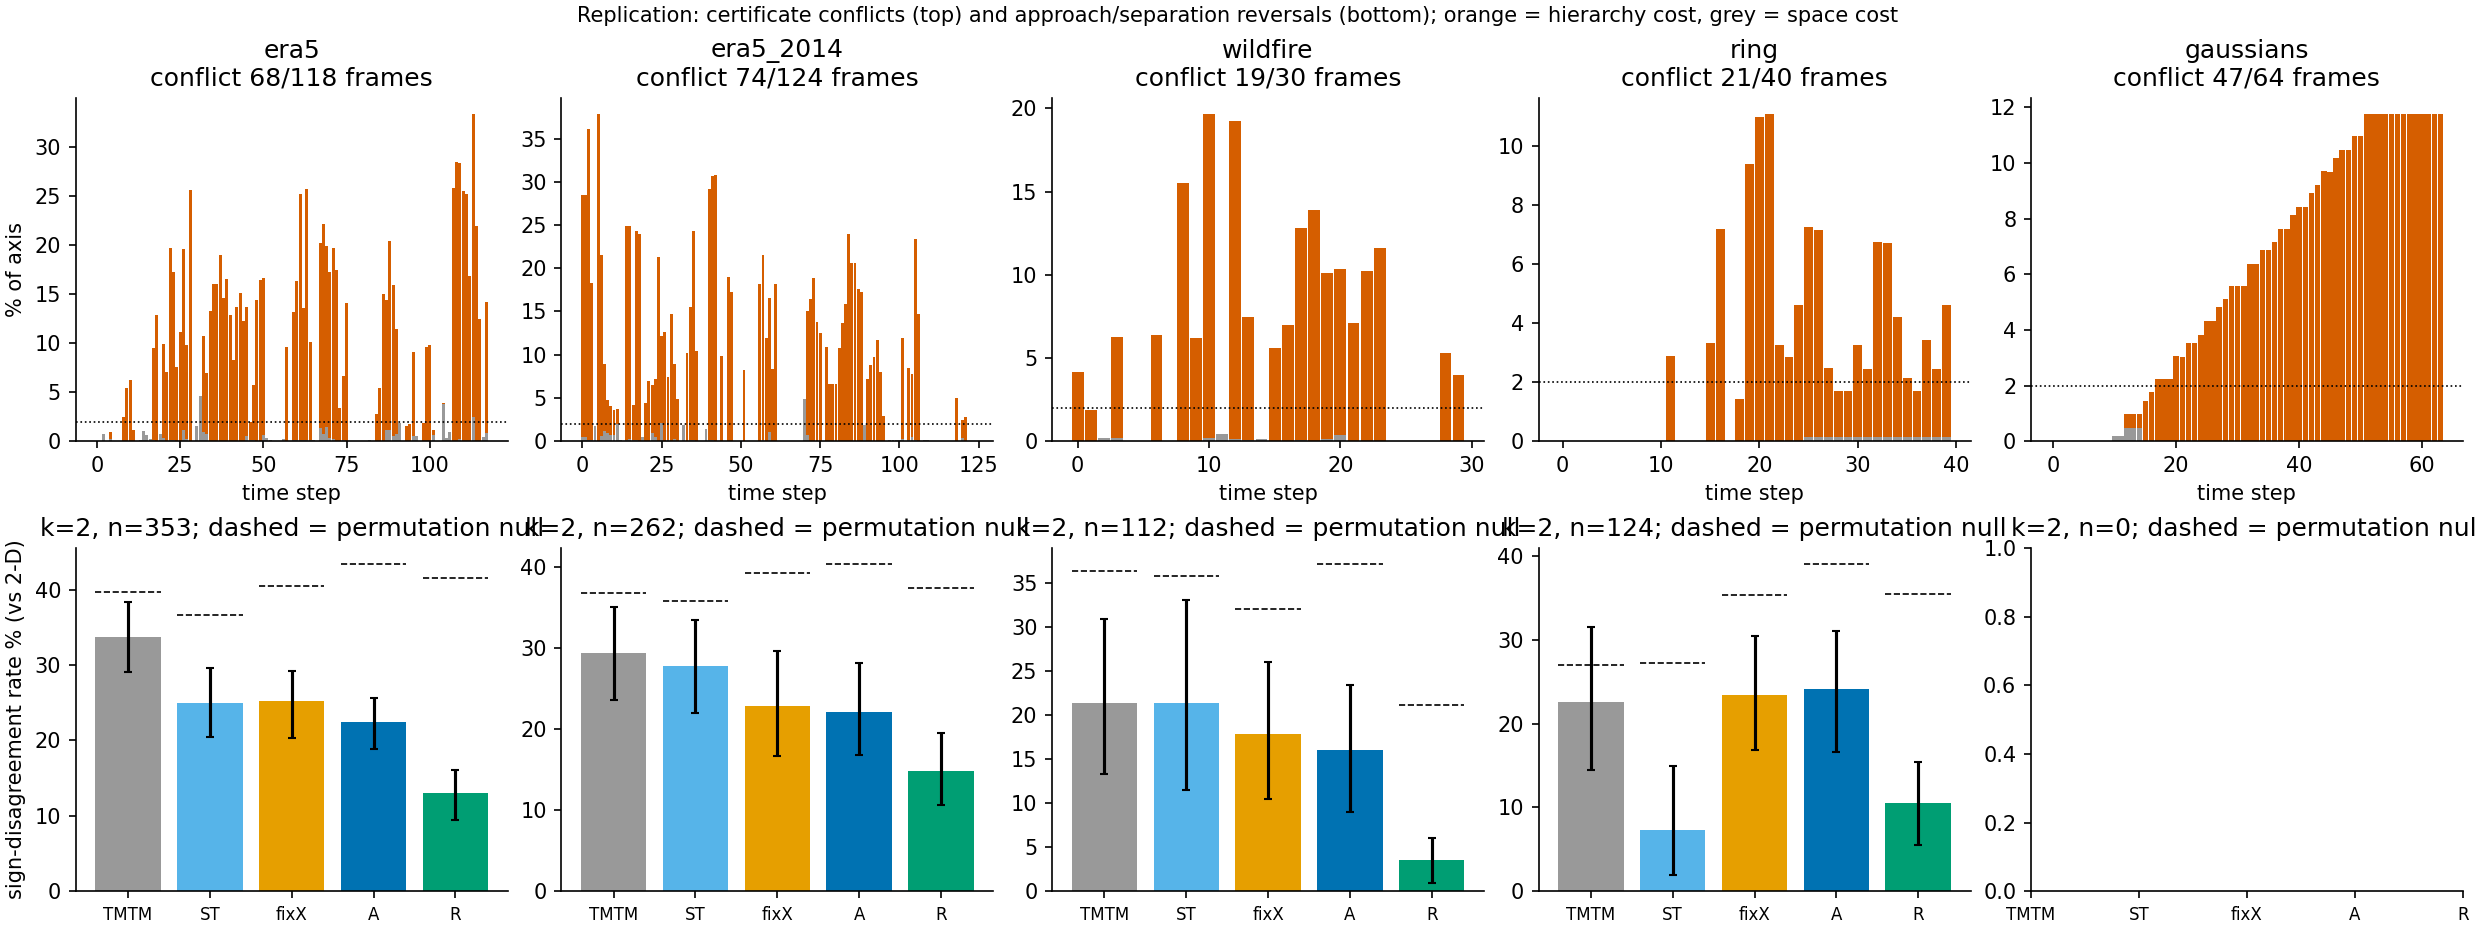
\includegraphics[width=\linewidth]{replicate_overview}
\caption{Top: per-frame space cost $\tau_{\rm free}$ (grey) and hierarchy cost $H$ (orange) in \% of the axis; dotted line: $\theta$. Bottom: sign-disagreement rates of the geometric reader proxy with 95\% intervals; dashed: permutation null.}
\label{fig:overview}
\end{figure*}

\textbf{RQ2: What does the conflict do to motion readings?}
A proxy reads a pair of tracks as approaching or separating when their map distance changes by more than 2\% of the occupied anchor range; the truth is the change of their 2-D extremum distance beyond 2\% of the domain diagonal. A \emph{reversal} is a clear truth read as the clear opposite; a \emph{miss} is a clear truth read as no change. Differences between methods use a paired bootstrap over 8-frame blocks. \Cref{tab:proxy} shows that the relaxed map reverses significantly less often than ST-MTM on all three real datasets (differences of $-11.9$, $-13.0$, and $-17.9$ points; intervals exclude zero) and also misses less on ERA5, but misses more on fire ($+15.2$ points). On Ring the difference to ST-MTM is not significant. The ranking is stable for reader thresholds of 1\%, 2\%, and 5\%. Keeping the hierarchy (A) performs like ST-MTM; only relaxation helps, consistent with the corollary. This is a geometric diagnostic that knows feature identities and anchor coordinates, not a study of human readers.

\begin{table}[t]
\centering\small
\begin{tabular}{lrcccc}\toprule
Data & $n$ & TMTM & ST-MTM & A & R\\\midrule
ERA5 & 353 & 33.7 & 24.9 / 27.2 & 22.4 / \phantom{0}9.3 & \textbf{13.0} / \phantom{0}7.1\\
ERA5-14 & 262 & 29.4 & 27.9 / 26.7 & 22.1 / 17.2 & \textbf{14.9} / 17.9\\
Fire & 112 & 21.4 & 21.4 / 14.3 & 16.1 / 16.1 & \textbf{3.6} / 29.5\\
Ring & 124 & 22.6 & \textbf{7.3} / 27.4 & 24.2 / \phantom{0}7.3 & 10.5 / \phantom{0}2.4\\\bottomrule
\end{tabular}
\caption{Reversal / miss rates (\%) of the geometric reader proxy over 24-hour windows (fire: four days). TMTM misses are omitted for space.}
\label{tab:proxy}
\end{table}

\textbf{RQ3: What does fidelity cost, and is the relaxation optimal?}
\Cref{fig:frontier} shows, per dataset, the exact attainable frontier $F$ (Theorem~\ref{thm:exact}), the certified bound $\Phi$, and our layouts. Theorem~\ref{thm:price} holds in all 924 frames with broken contiguity, and no layout lies below $\Phi$ or $F$. At a merge-gap budget of 2\% of the value range, relaxation lowers the mean reference error by 11--13\% on pressure at 1.4--2.1\,hPa of merge distortion with the optimal filling (2.5--2.7\,hPa with the LCA filling), but by 45\% on fire; at 20\%, by 59--74\% on pressure at 28--32\,hPa. The cost of positional fidelity depends on the merge structure: fire conflicts stem from weak merges between neighbouring hot spots, pressure conflicts from strong saddles and shallow lows.

\emph{Optimality.} Per frame, the pair $(\tau(\pi),\delta^*(\pi))$ of the relaxed order lies on the exact frontier within half a pixel in 368 of 376 frames at $\kappa=2\%$ and in at least 90\% of frames of every dataset and budget; it is never more than 0.7\% of the axis above it. The aggregate points in \cref{fig:frontier} lie above $F$ because the budget selects nodes by $\gamma_v$, whereas the exact cost $\delta^*$ also contains the leaf-height term, so frames spend less than the global budget.

\emph{Tightness of the certified bound.} $F-\Phi$ averages 0.3--2.3\% of the axis over all breakpoints of $\Phi$ and is within half a pixel at 29--36\% of them; it exceeds 10\% in a few pressure and fire frames (at most 25\%). $\Phi$ ignores the leaf-height term of Proposition~\ref{prop:fill}, which can only widen this gap. The optimal filling halves $d_{\rm top}$ where only merge gaps matter (Ring, Gaussians) but saves little on pressure at large budgets, again because of shallow lows.

\begin{figure*}[t]
\centering
  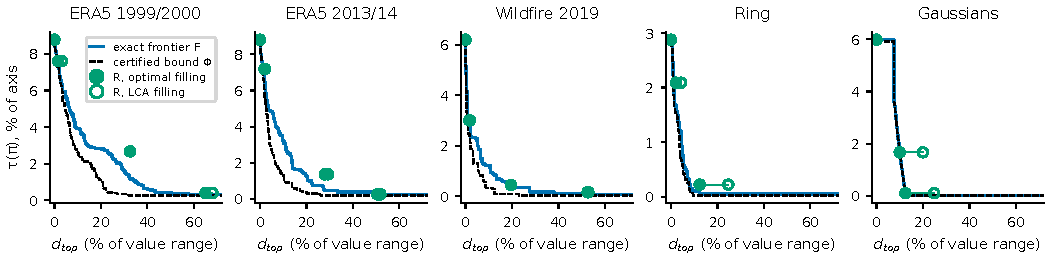
\includegraphics[width=\linewidth]{fig_frontier_exact}
\caption{Position--topology trade-off per dataset: exact attainable frontier $F$ over all 1-D maps (blue, Theorem~\ref{thm:exact}), certified lower bound $\Phi$ (dashed, Corollary~\ref{cor:frontier}), and certificate-driven relaxation for budgets $\kappa\in\{0,2\%,20\%,\infty\}$ with the optimal filling (filled) and the LCA filling (open). $x$: maximum over frames of $d_{\rm top}$; $y$: mean over frames of the maximum position error.}
\label{fig:frontier}
\end{figure*}

\textbf{RQ4: Does the certificate transfer?}
We ordered 1024 active 10-km fire cells, one pixel row each, by an agglomerative clustering of their fire time series, the hierarchy behind Franke et al.'s hierarchical orderings~\cite{Franke:2021:1DP}. The certificate shows that any order consistent with this dendrogram must displace some cell by at least 67\% of the display height from its geographic rank-scaled position; the hierarchy cost is 47--48\% for three linkages, versus 1.4\% for a spatial Ward dendrogram but 32.5\% for a spatial single-linkage dendrogram. With OLO, cells sit up to 88\% (median 14\%) away from geography (\cref{fig:dendro}). The certificate thus answers a design question before anyone reads geography off a clustered display: here, ``row position approximates location'' is untenable, and a linked map view or a spatially constrained hierarchy is required. The exact computation takes 0.1\,s.

\begin{figure*}[t]
\centering
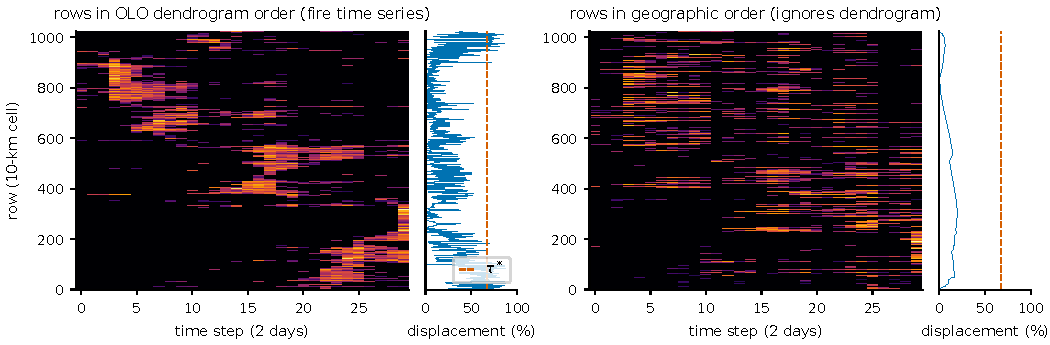
\includegraphics[width=\linewidth]{dendrogram_demo}
\caption{1024 wildfire cells (rows) over two months (columns) ordered by an optimal-leaf-ordered dendrogram of their fire time series (left) and by geography (right). OLO displaces cells by up to 88\% of the display height from their geographic position; the certificate proves that no dendrogram-consistent order can do better than 67\%.}
\label{fig:dendro}
\end{figure*}

\section{Discussion and Limitations}
Our results suggest three practices for hierarchy-constrained 1-D displays: keep the hierarchy by default and disclose the certified deviation; relax explicitly when position matters and show the topological cost; and report achieved error relative to the certificate when proposing new layouts.
The reader proxy is geometric; human judgements may differ. The width-free certificate covers the native width models of TMTM and ST-MTM, but the reader proxy compares methods that optimize different objectives, and ST-MTM parameter sensitivity is not studied. Relaxation has no approximation guarantee, although it is on the exact frontier in almost all frames; the exact frontier requires enumerating $n!$ orders, and the scalable bound $\Phi$ ignores the leaf-height term. The dynamic program is pseudo-polynomial and exponential in node degree, and layout selection still enumerates orders. A single reference direction cannot encode orthogonal motion. We also report negative results: automatic radial centres followed tracking artefacts, a stability-priority policy did not generalize, and per-feature disclosure ticks were illegible on ERA5.

\section{Conclusion}
We certified how far hierarchy-constrained 1-D layouts must deviate from a positional reference, proved a filling-independent topological price for breaking contiguity, and derived a certified position--topology frontier. Across two domains, hierarchy conflicts are common, can reverse motion readings, and cost a data-dependent amount of topology to resolve.

\section*{Supplemental Materials}
\label{sec:supplemental_materials}
The supplement contains complete proofs of all statements, the code to reproduce every experiment and figure, and the processed feature data. \todo{anonymized archive link}

\section*{Figure Credits}
\label{sec:figure_credits}
All figures were created by the authors. Fire data: Franke et al.~\cite{Franke:2021:1DP}, CC BY 4.0. ERA5: Copernicus Climate Change Service~\cite{Hersbach:2020:ERA5}.

%\acknowledgments{...}   % omitted for double-blind review

\bibliographystyle{abbrv-doi}
\bibliography{refs}
\end{document}
